\section{Ações de reação}
\label{sec:reacao}

Inicialmente, todos os comutadores possuem suas tabelas de encaminhamento vazias.Sendo assim, ao receber um pacote ocorre um \textit{table miss} e o pacote é encaminhado para o controlador através de uma mensagem \textit{Packet In}.

O controlador por si só, não realiza operações sobre a mensagem recebida, por isso, foi desenvolvido juntamente com este IPS, um interpretador de mensagens \textit{Packet In}. Este analisa os dados do cabeçalho do pacote obtendo as informações de origem e destino do fluxo e os compara com os endereços armazenados na lista de endereços maliciosos para descarte. Dependendo do resultado, o controlador poderá adicionar no \textit{switch} uma regra de encaminhamento o ou tomar uma ação de prevenção, adicionando uma regra para descarte do fluxo.

Mensagens para alteração da tabela de encaminhamento podem ter os seguintes tipos:
\begin{itemize}
    \item \textbf{OFPFC\_ADD} - Adiciona um novo fluxo;
    \item \textbf{OFPFC\_MODIFY} - Modifica entradas de fluxo existentes;
    \item \textbf{OFPFC\_MODIFY\_STRICT} - Modifica entradas de fluxo existentes validando estritamente seus campos, ou seja, apenas uma entrada da tabela é modificada;
    \item \textbf{OFPFC\_DELETE} - Remove entradas de fluxo existente; e
    \item \textbf{OFPFC\_DELETE\_STRICT} - Remove entradas de fluxo validando estritamente seus campos, ou seja, apenas uma entrada da tabela é removida.
\end{itemize}

Entradas de fluxos podem ser removidos da tabela de encaminhamento por três maneiras: através da requisição do controlador, pelo mecanismo de \textit{timeout}, ou pelo mecanismo de despejo opcional. O mecanismo de \textit{timeout} é executado pelo \textit{switch} independentemente do controlador e é baseado na configuração e no estado das entradas de fluxo. Neste trabalho, foi definido um intervalo de \textit{timeout} para cada fluxo para que não ocorra \textit{overflow} de regras nas tabelas de encaminhamento. Um fluxo só permanecerá na tabela por um pequeno intervalo após o recebimento de seu último pacote.

Para alterar ou remover alguma entrada da tabela de fluxo, deve ser enviada uma mensagem do tipo OFPT\_FLOW\_MOD que é definida conforme ilustra a Figura \ref{fig:ofp-flow-mod}.

\begin{figure}[H]
  \centering
  \caption{Corpo da mensagem de alteração de entradas na tabela de fluxo.}
  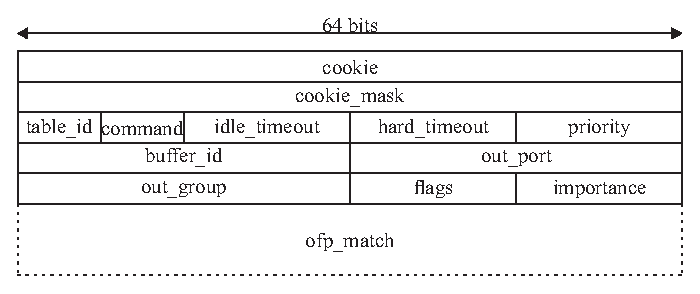
\includegraphics[width=.80\textwidth]{images/ofp-flow-mod.eps}
  \label{fig:ofp-flow-mod}
  \fonte{\centering Elaborado pelo autor a partir de informações da especificação OpenFlow.}
\end{figure}
O campo \textit{table\_id} refere-se à tabela a ser atualizada, que pode ser por fluxo, porta, como já citado. O campo \textit{command} refere-se á ação a ser executada (adição, alteração e remoção), campos \textit{timeout} indicam o tempo máximo de espera por um fluxo antes do descarte, \textit{priority} armazena a prioridade da entrada na tabela de fluxo. O campo \textit{ofp\_match} indicam as regras de encaminhamento de fluxos. Os demais campos não serão abordados neste mas seu estudo pode ser realizado através especificação OpenFlow \cite{OpenFlowSpec:2014}.

Alterando a regras de encaminhamento através destas mensagens, além de reagir ao ataque em questão, o sistema também estará protegido contra novos fluxos de mesma origem, sem a necessidade de consultar o controlador.

Algumas medidas de prevenção também foram preestabelecidas no controlador. Por padrão toda conexão não maliciosa, deve iniciar a comunicação com um pacote SYN. Sendo assim, ao receber um pacote com \textit{flag} diferente da SYN, o controlador imediatamente descarta o pacote, prevenindo assim o ataques do tipo ACK, exploração FIN e Xmas Tree.

Os fluxos adicionados pelo controlador nas tabelas de encaminhamento possuem como regras as informações chave do cabeçalho mencionadas, desta forma, cada fluxo recebido irá possuir uma única entrada na tabela. Neste instante é também configurado um \textit{timeout} para este fluxo. Este \textit{timeout} foi estabelecido em quinze segundos, tempo permite que o fluxo não seja removido da tabela caso houver um pequeno atraso na transmissão dos pacotes além possibilitar que coletas de estatísticas sejam realizadas, pois uma vez removido o fluxo, não é mais possível obter suas informações. O Quadro \ref{fll}, ilustra uma tabela de fluxo com as regras utilizadas pelo \textit{software} proposto, regras não utilizadas foram omitidas da tabela para melhor leitura.

\begin{table}[H]
\centering
\caption{Exemplo de fluxos na tabela de encaminhamento.}
\resizebox{\textwidth}{!}{
\label{fll}
\begin{tabular}{|c|c|c|c|c|c|c|c|}
\hline
\multicolumn{5}{|c|}{REGRAS}                           & AÇÃO       & PRIORIDADE & TIMEOUT       \\ \hline
type & src\_ip    & dst\_ip    & src\_port & dst\_port &            &            & idle\_timeout \\ \hline
TCP  & 10.0.0.11  & 10.0.1.124 & 36987     & 80        & encaminhar & 50000      & 15            \\ \hline
TCP  & 10.10.0.45 & 10.10.2.43 & 23234     & 80        & encaminhar & 50000      & 15            \\ \hline
TCP  & 10.0.0.114 & 10.10.2.29 & 35455     & 22        & encaminhar & 50000      & 15            \\ \hline
TCP  & 10.10.2.24 & 10.0.0.12  & 32444     & 25        & descartar  & 50000      & 0             \\ \hline
\end{tabular}}
\fonte{\centering Elaborado pelo autor.}
\end{table}

Neste exemplo, os três primeiros fluxos são de encaminhamento e foram criados com um \textit{idle\_timeout} de quinze segundo. Se nenhum novo pacote desse fluxo for recebido nesse intervalo de tempo, o fluxo é removido da tabela de encaminhamento. O quarto fluxo é de descarte, ou seja, quando for recebido um fluxo onde os campos de cabeçalho dos pacotes correspondam aos campos das regras, o mesmo será descartado. Este último possui um \textit{timeout} nulo, o que significa que a regra é permanente e, se necessário for, deverá ser removida da tabela através de uma mensagem do controlador.

A natureza de visão global da rede possibilitada por \gls{sdn} permite que a aplicação faça a detecção de \text{switches} individuais e envie fluxos de descarte para os demais, impossibilitando que tais fluxos tomem rotas diferentes para o \textit{host} alvo. Além disso, controladores distintos podem efetuar a troca de informações referentes a fluxos de varredura de porta, possibilitando a proteção de outras redes não gerenciadas pelo mesmo controlador.








